\cleartorightpage
\begin{savequote}[75mm]
If you don't know where you're going, you might not get there.
\qauthor{Yogi Berra}
\end{savequote}


\chapter{Introduction and Outline}\label{introduction}
 % start numberings at 0 because (computer) science
\setcounter{figure}{-1}
\setcounter{table}{-1}
\setcounter{section}{-1}
\setcounter{NAT@ctr}{-1}

\setlength\parindent{0pt}

\section{Bioinformatics: A Solitary Pursuit?}

When one thinks of bioinformatics, one often thinks of the specific silo of
bioinformatics that is interesting to them, perhaps a specific analysis, or a
specific field. This focus on a single node in the network of bioinformatics
hides a lot of the complexity and cross-domain interactions that are not only
possible but required.

Linear pathways can be drawn in bioinformatics, from data to analysed product,
or from sequencing to differential expression analysis, but these obscure the
networks of topics and fields and analyses that exist outside of those yellow
brick roads, those happy paths. The reality is that the field of bioinformatics
look more like the most complicated biosynthesis pathway one can imagine. It's
full of interconnections between the traditionally included bioinformatics,
laboratory science, chemistry, but also to education and didactic theory, data
management planning, bioethics, code management, source control systems,
publishing. It is these second set of connections that aren't often considered,
but are a prerequisite for functioning science.

Take for instance a typical RNA-Seq analysis, generally this is summarised with
a very simple flowchart like \cref{rnaSeqSimple}. Ask a bioinformatician,
you'd probably get this answer which, while correct, is not complete.

\begin{figure}[!h]
\hypertarget{rnaSeqSimple}{%
\centering
\begin{tikzpicture}[node distance = 2cm, auto]
    \node [block] (map) {Splice Aware Mapping};
    \node [block, right=1em of map] (count) {Counting};
    \node [block, right=1em of count] (diffex) {Differential Expression};
    \node [block, right=1em of diffex] (viz) {Visualisation};
    \node [block, right=1em of viz] (go) {GO Enrichment};
    \node [block, right=1em of go,below=1em of go] (path) {Pathway Analysis};
    \path [line] (map) -- (count);
    \path [line] (count) -- (diffex);
    \path [line] (diffex) -- (viz);
    \path [line] (viz) -- (go);
    \path [line] (viz) -- (path);
\end{tikzpicture}
\caption{A simplified RNA Seq workflow. TODO: fix graphic.\label{rnaSeqSimple}}
}
\end{figure}

This simplified view hides a lot of very important aspects of responsible
science\cite{NAS1992} such as where is one running these computations? Is it
reproducible? Where did they learn to do it? What's the data management plant?
Is it ethical?

All of these topics are part and parcel of the scientific process, especially in
biomedical sciences, but too often ignored for a focus on translational research
and clinical applications. So let's look at the ``real'' flow chart of doing a
simple differential expression analysis instead.

\begin{figure}[!h]
\hypertarget{rnaSeqNotSoSimple}{%
\centering
	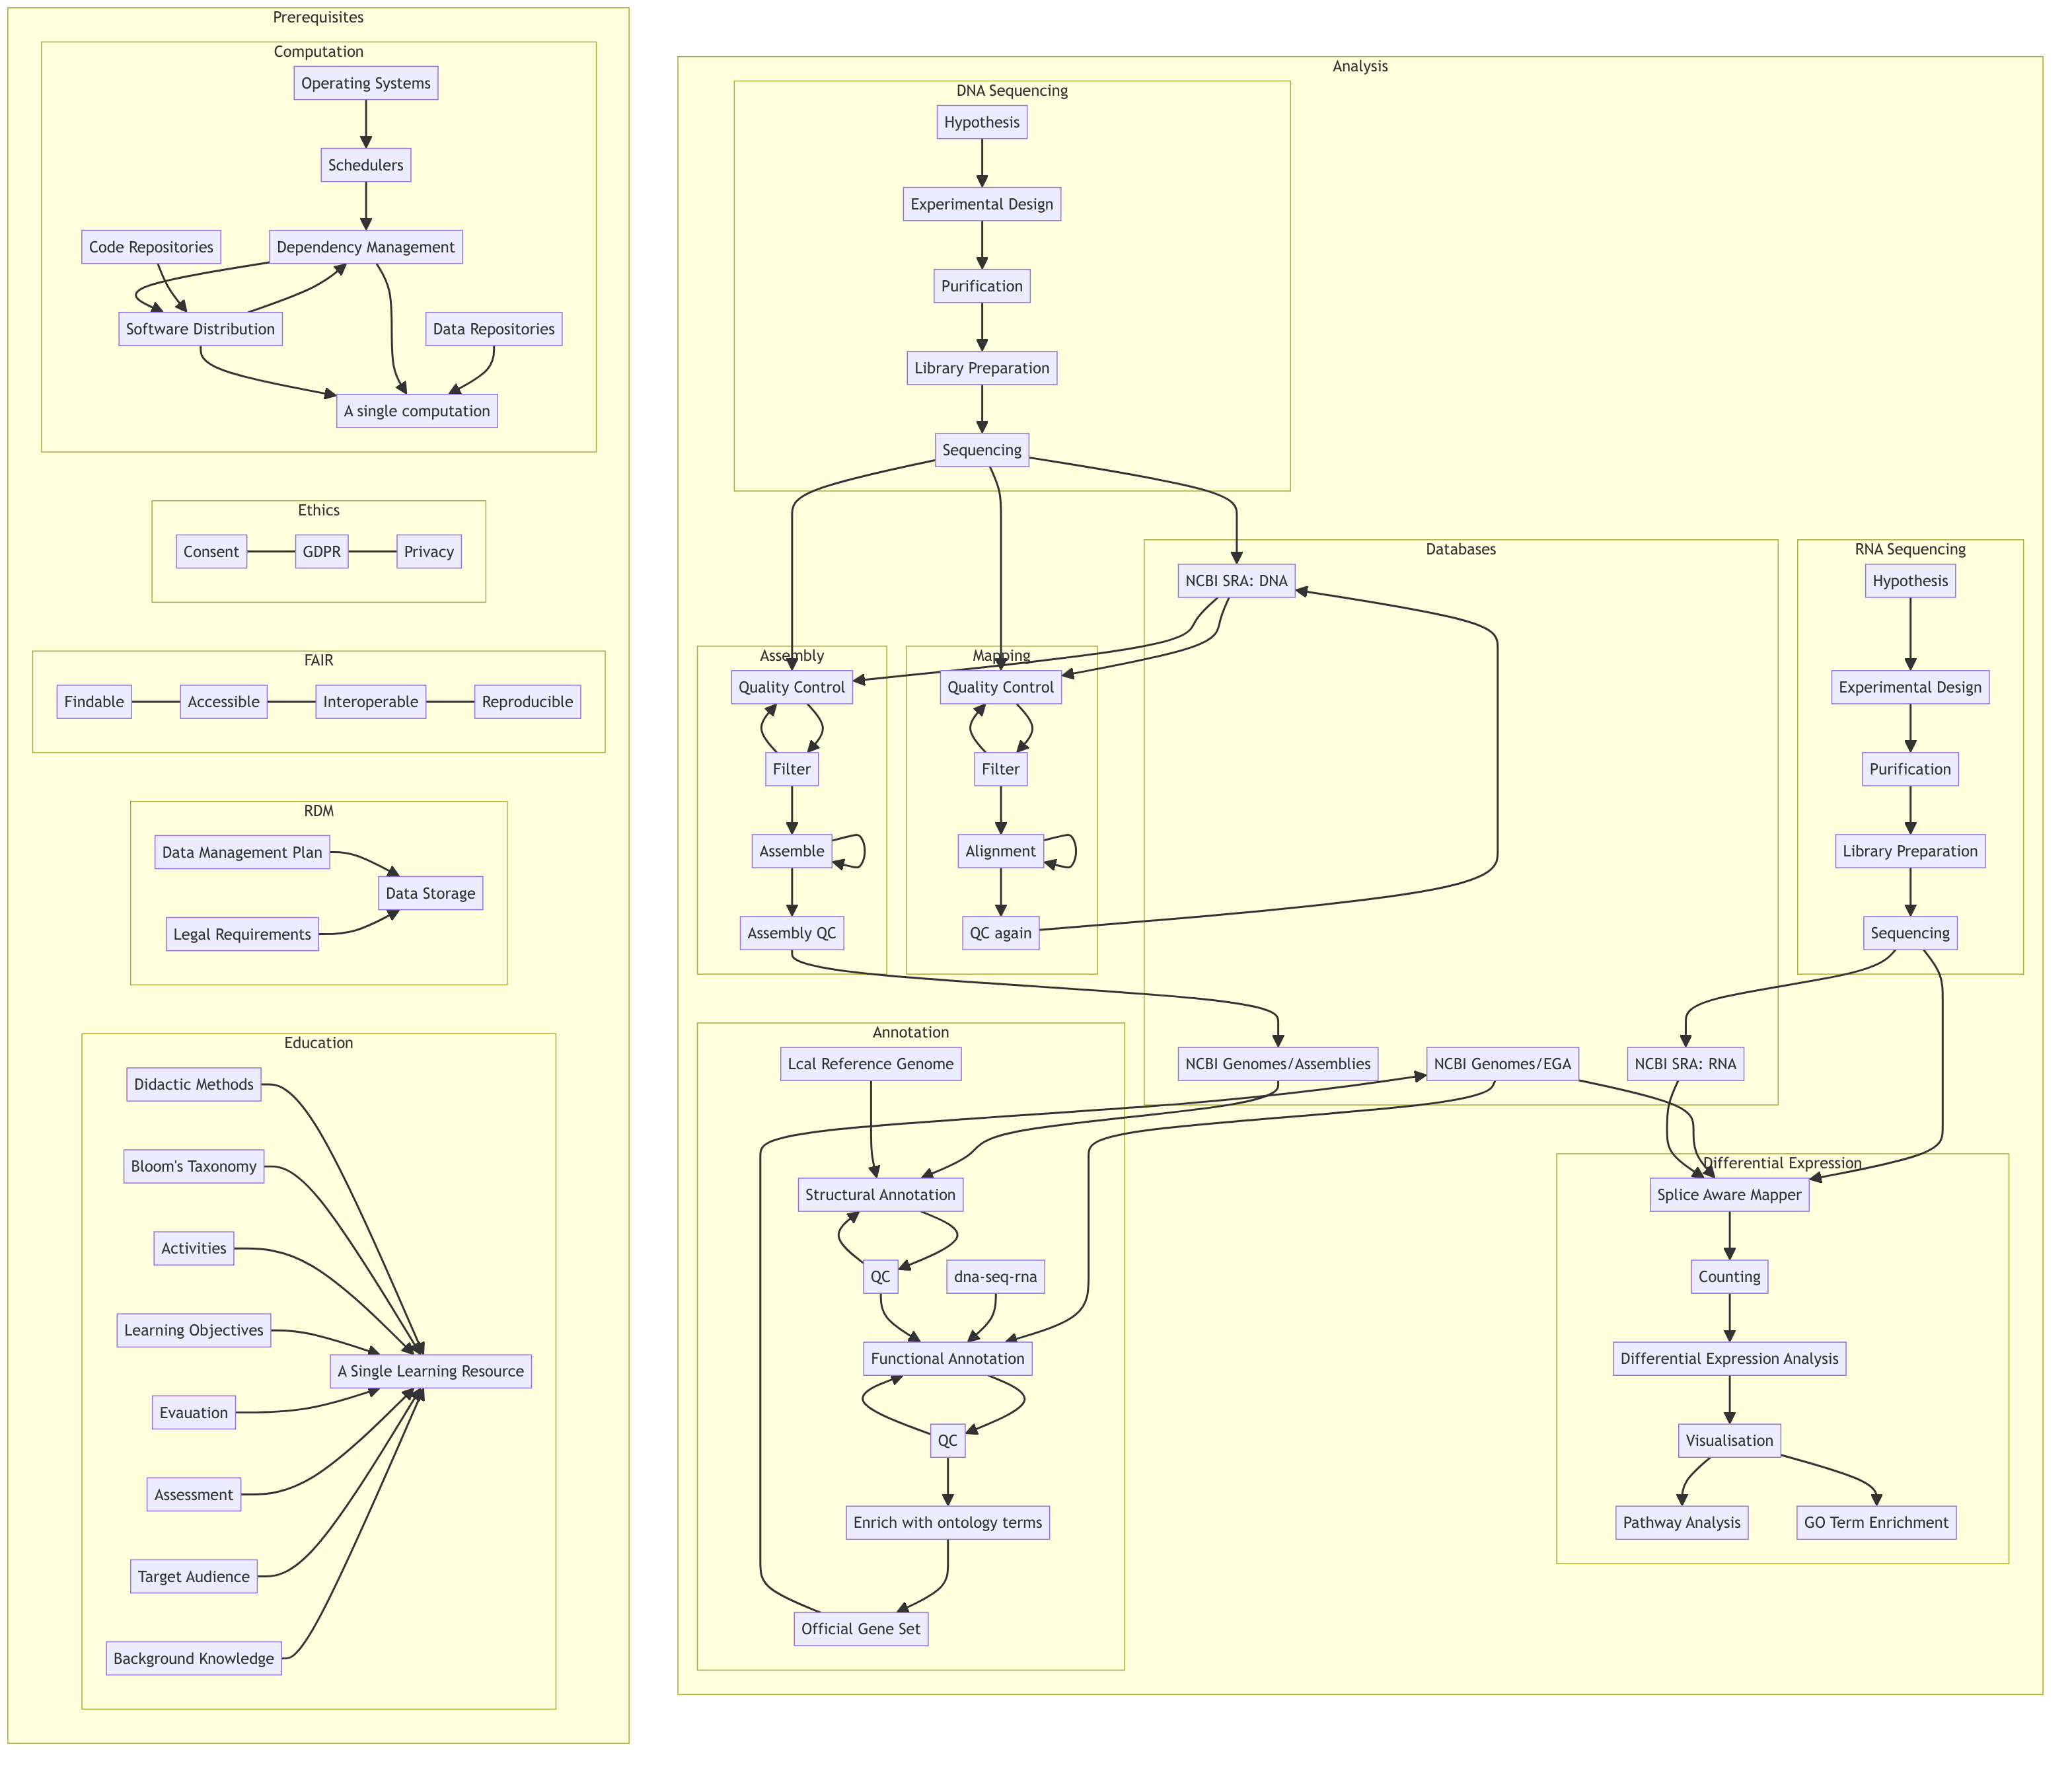
\includegraphics[width=\textwidth]{./mermaid/diag.mmd.png}
	\caption{A ``simplified'' RNA Seq workflow. TODO: fix graphic, colours.}\label{rnaSeqNotSoSimple}
}
\end{figure}

\Cref{rnaSeqNotSoSimple} shows a more accurate view of the simple analysis.
Every single aspect of the process, from start to end, builds on learning
materials and resources. When created by professionals, their creation is an
involved and complicated process to produce a high quality learning resource.
Someone, somewhere, needed to learn the requisite skills to complete their
subset of the workflow. Additionally many of the steps are computational in
nature, which requires we ask questions regarding the computations such as which
Operating System (OS), Distributed Resource Manager (DRM), and dependency
management system were used? These are all important for the reproducibility of
the analysis, and are as important as the research results in order to avoid
situations like the Polderman affair by providing a traceable chain of analyses
that is reproducible now, \emph{and} at a later date.

This thesis touches on these topics, identifying and implementing
solutions to support and improve the quality of science done by
bioinformaticians who are more focused on clinical outcomes.

% We'll begin with the computational infrastructure, the oft-ignored foundation of
% bioinformatics in medicine. With that in hand we'll move into the bioinformatics
% itself, focusing first on genome annotation, the again oft-ignored foundation of
% all analyses. This provides the basis for discussing scientific applications and
% work to improve translational research. This grimoire is then concluded with a
% discussion of training, how we can disseminate the spells and rituals (tools and
% analyses, if you prefer) to a wider audience.
%
% After all, what use is a tool that falls in a forest, or is released online
% without proper documentation and learning materials?

\section{Paying the Bioinformatics TARRIIF}

FAIR has been a key concept in bioinformatics since 2016. It is a vital
component in making sure our research does not go to waste. By requiring FAIR
data funders help ensure that datasets are: Findable, Accessible, Interoperable,
and Reusable.

Additionally some have added a second R: Reproducibility. This aims to
highlight and address the reproducibility crisis within science. If we have
truly FAIR datasets, we should be able to easily reproduce the research.

This updated acronym falls short on two fronts: \emph{Teaching}, and
\emph{Infrastructure}.

Bioinformatics is a rapidly growing field, but the growth in data is far
outpacing the growth in researchers. Advancements in sequencing mean that we
generate NUMBER PB of data every TIME PERIOD which must be analysed.
Unfortunately researchers do not scaling at the same rate as the data.

It is a classic economics problem, the supply of humans to accomplish research
is significantly lower than the demand. The demand continues to grow putting
pressure on the supply chain for bioinformaticians, pushing us to find ways to
make bioinformatics, and bioinformaticians, more scalable.

Naturally we should examine this through a systems lens: what levers are
available to us which can change the inputs or outputs of the system to match
our desired goal? We can turn the compute lever, making compute resources more
available to researchers via efforts like the \#EuroHPC JU. Or maybe we should
place pressure on making tooling more cost efficient. Can we increase the supply
of students coming in to bioinformatics programs?

As others focus on the availability of tooling and workflows, what if we instead
considered focusing on these points? Improving the availability and
accessibility of infrastructure, and decreasing barriers in order to accelerate
the supply of required bioinformaticians.

% What should be made of a dataset for an uncommon research project that cannot
% leverage community standards and resources. It might be FAIR, even FAIRR if
% there is a pipeline generating it, but without documentation and training
% materials associated with the resource describing the generation process it
% becomes prohibitively costly to engage with an unknown dataset. Without
% infrastructure on which to analyse the data, it will sit unanalysed.


\section{Going where FAIR hasn't gone before}

Once we've paid the TARRIIF, we've set a baseline for the resources we produce
as part of our scientific efforts. It it the \emph{bare} minimum, nowhere near
the maximum. There are areas where we can choose to go above any beyond the
minimum requirements for good science.

\subsection{Accessibility}

% Not just accessible but easily!
% - even when tools exist, accessibility issues are abound
% - two kinds: disability access + availability
% - does a given tool work for a blind user?
% - can it be accessed around the world? in non-LMICs?

The term accessibility is overloaded, there are multiple understandings which
are often conflated; access to a resource, and access for those with
disabilities. Making bioinformatics accessible, in both senses, must be our
goal. How can we make resources we maintain, available to the entire world,
and without barriers?

Can we make the compute resources available in High Income Countries (HICs),
generally the ex-colonial powers, available to those in Low and Middle Income
Countries (LMICs)? Can we make our carefully guarded knowledge available around
the world? Can we optimise the computations to require less energy and compute
time? When these resources are available, are we actively excluding this with
one or more disabilities from engaging with the materials and tools?

The answer presented in this thesis is a resounding ``yes, we can do it''. Not
only are the tools and workflows and infrastructure made freely available, both
free-as-in-beer\footnote{I.e. the recipe is available, you can make it
yourself}, and free-as-in-grant-funded for many of the resources we put online.
Resources discussed in this thesis were disseminated globally to around 7.500
students over the last 3 years of my PhD employment. All of these resources were
made available barrier-free with extra consideration for their accessibility in
the cases of visual or auditory impairments. It's possible, even easy, one just
needs to put in the effort and value those community members.

\subsection{Automation}

No discussion of scaling resources is complete without consideration for
opportunities to automate existing processes; depending on the frequency and
time costs of a task, one can examine the return on investment for automating it
(\cref{xkcdautomate}).

\begin{figure}[!h]
\centering
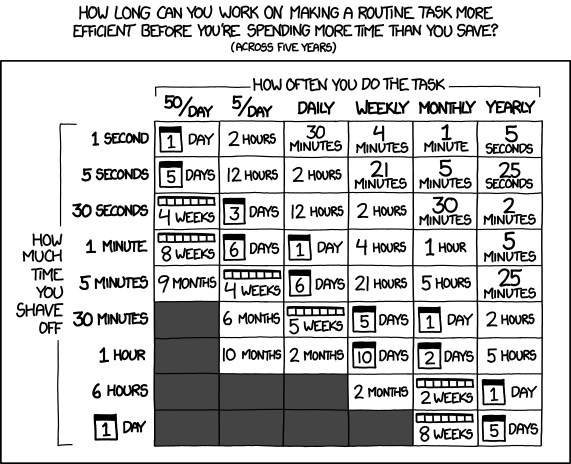
\includegraphics[width=0.8\linewidth]{chapters/images/introduction/is_it_worth_the_time.png}
\caption{Figure reproduced from XKCD \#1205. This work is licensed and
	reproduced under a Creative Commons Attribution-NonCommercial 2.5
	License.\label{xkcdautomate}}
\end{figure}

Return on investment is a rather capitalistic lens through which to discuss the
topic, but a logical one in medicine. Not every task is easy to automate and
thus worth a large time investment, nor every task worth automating if the
savings are marginal.

This analysis dovetails with our systems view; which levers do we have access
to, and where can we have effects. Every chapter of this thesis attempts to
automate or improve the existing automation of processes: infrastructure
management and administration, annotation of genomes, translational research
and clinical reporting, and finally teaching.

% \section{Teaching}
%
% \section{404: Help Not Found}
% % - bioinformatics is difficult
% % - bioinformaticians and not really scalable
% % - people need our resources, we need to make them available
% % - And we need to make training available
%
%
% \section{Automating Bioinformatics}
% - When it is available, does it scale?
% - Can parts be automated, to reduce demands on humans?
%
% \begin{figure}[!h]
% \centering
% 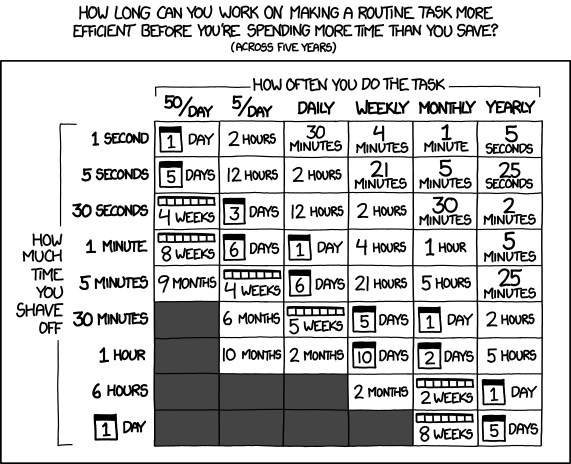
\includegraphics[width=0.8\linewidth]{chapters/images/introduction/is_it_worth_the_time.png}
% \caption{Figure reproduced from XKCD \#1205. This work is licensed under a Creative Commons Attribution-NonCommercial 2.5 License.}
% \end{figure}
%
% \section{Use case 1: Cancer}
% - circos makes nice plots that are useful for cancer
% - it's available in CancerGalaxy™®, which collects other useful tools + training
% - (maybe) here's a more science-y example: htsget for analysis
% - (maybe) here's another science-y reproduction: pathways
% - and finally real life translational medicine: (EC-PC/Arlene/Etc, whatever works out.)
%
% \section{Use case 2: Annotation}
% - Galaxy Genome Annotation project makes scalable genomics easy, plus teaching.
% - Apollo brings collaborative annotation, for teaching + science
% - (maybe) Tripal puts genomes in front of scientists
% - Phages have some health applications, here we talk about annotating + teaching.

% \section{Aim of the Thesis}

\section{Scope of this Thesis}
In \cref{chapter:platform} we present three highly integrated components as a necessary basis for the rest of the thesis. Galaxy, a platform on which to scale one's research, from learning and small courses to full fledged research projects. This is complemented by Planemo, a toolkit for developing reproducible workflows and tooling with which to use in Galaxy. And finally we scale the TIaaS platform, which we use to address the needs of trainers by providing infrastructure as-a-service, reaching 24.000 researchers over the past 5 years.

Next in \cref{chapter:annotation} we look at the annotation of genomes, a necessary pre-requisite step in any and every downstream analysis, especially in medical contexts. We harken back to the first chapter by presenting a platform for scalable, real-time genome annotation, and then demonstrate the use of this platform in the annotation of phages, a topic of growing interest in the medical community. We also present the work of an ontology based toolkit for FAIR community databases, ensuring high quality computationally analysable annotations are recorded and distributed. % Finally we summarise all of this infrastructure work by making our genome annotation infrastructure easily re-deployable by other groups via the GGA docker containers.

With a truly scalable, FAIR platform in place we next look at the connection to
the medical research world, specifically translational research in \cref{chapter:cancer}.
%We demonstrate this by deploying a number of bioinformatics tools import for Cancer on our platform and making them available globally.
We open on the problem of where to obtain data, necessitating the integration of the European Genome Archive (EGA) in a secure manner, allowing for end-to-end analysis of sensitive clinical data.
Next presenting a clinical application of Galaxy with the analysis of EC-PC data.
Finally we visualise our results, showcasing a commonly used visualisation tool within cancer genomics; Circos.

With three chapters of reproducible, scalable analyses the only remaining
question is how to ensure they reach their audience. As we benefit at every step
from the existing learning materials produced by educators around the world, we
give back by building a scalable training platform. Thus we share the updates to
our scalable, FAIR, and accessible training platform which has been improved
over the last two years in \cref{chapter:training}. These improvements would
prove key as the SARS-CoV-2 pandemic isolated the world, we were able to
leverage the platform and training infrastructure to rapidly respond to the
needs of the community, namely providing an e-learning platform.



A lot of our esteemed colleagues have focused on the bioinformatics of cancer
itself as well as clinical solutions to the problem. We instead aim to focus on
the platform, infrastructure, and training aspects of clinical research. This
presents a unique opportunity to act as a force multiplier for the field, by
making the tools and training more accessible to the world. With our platform we
can scale the equally important work of our colleagues, reaching tens of
thousands of researchers.

After all, what use is a tool that falls in a forest? (or is released online
without proper documentation and learning materials?)

\footnotesize
\bibliographystyle{ieeetr}
\bibliography{references}
\normalsize
